\begin{frame}
\frametitle{Обучение с подкреплением}
\begin{columns}
\column{0.4\linewidth}
  \centering
  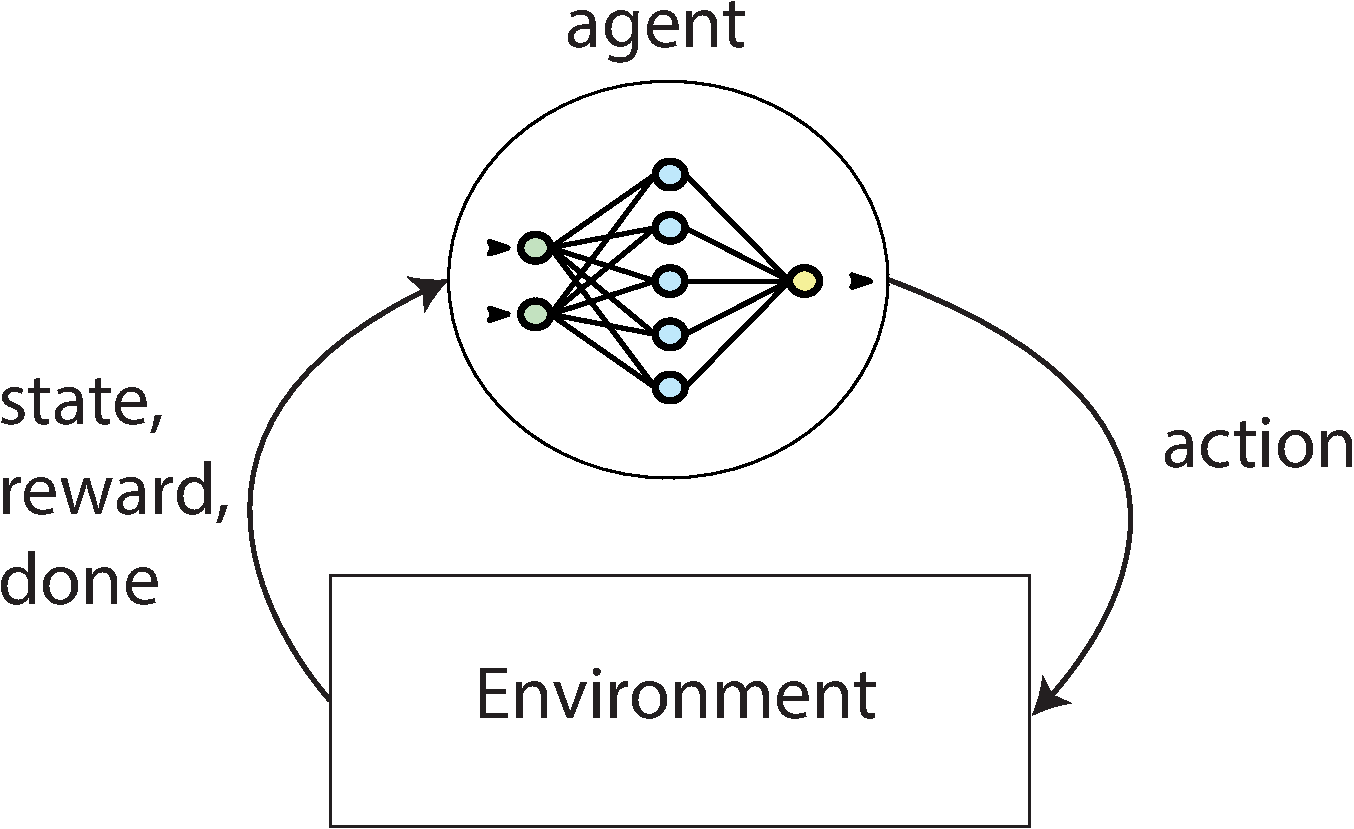
\includegraphics[width=1\linewidth]{images/rl_setting.pdf}
  
  \begin{equation*}
    <\mathcal{S, A, R, P}, \gamma>
  \end{equation*}

\column{0.6\linewidth}


\begin{align*}
& \ex_{\tau \sim \pi_{\theta}} [J(\tau)] = \ex_{\tau \sim \pi_{\theta}} \left[r_0 + \gamma r_{1} + \gamma ^ 2 r_{2} + ...\right] \\
& V(s_t) = \ex\left[\sum \gamma ^t r_{t}\right] \\
& Q(s_t, a_t) = \ex\left[r_t + \sum \gamma ^{t + 1} r_{t + 1}\right] \\
\end{align*}
\end{columns} 
\end{frame}

\section{Настройка оптического интерферометра методами машинного обучения с подкреплением}

\subsection{Постановка задачи}

\begin{frame}
\frametitle{Физические принципы работы и модель оптического интерферометра}
\begin{columns}
\column{0.5\linewidth}
  \centering
  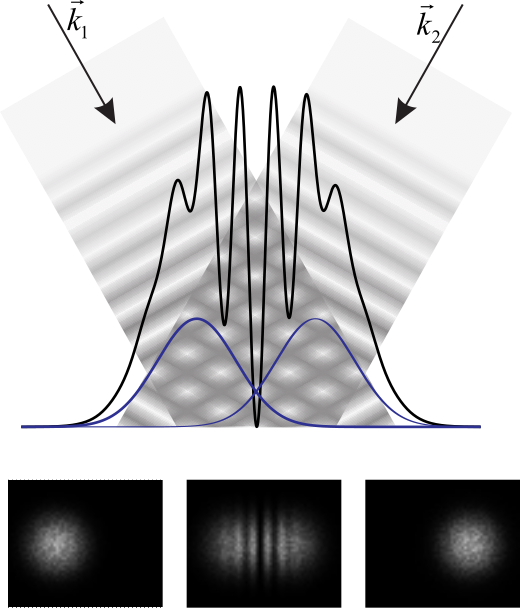
\includegraphics[width=0.9\linewidth]{images/interf_expl.png}

\column{0.5\linewidth}

\begin{align*}
& E(x,y,z)=\exp \left[-\frac{\left(x-x_{0}\right)^{2}+\left(y-y_{0}\right)^{2}}{r^{2}(z)}\right] \cdot \\
& \hspace{20pt} \exp \left[-i\left(k_{x} x+k_{y} y+k_{z} z + k\frac{x^2+y^2}{2\rho^2(z)} z\right)\right] \\
& E(x, y, z) = E_1(x, y, z) + E_2(x, y, z) \\
& I(x, y, z) = |E(x, y, z)|^2 = E(x,y,z) \cdot E^*(x,y,z) \\
& I= I_1 + I_2 + 2 \sqrt{I_1I_2}\cos(\Delta \phi)
\end{align*}

\end{columns} 
\end{frame}

\begin{frame}
\frametitle{Интерферометр Маха-Цендера}
  \centering
  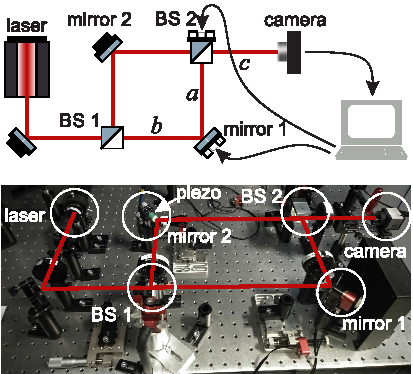
\includegraphics[width=0.8\linewidth]{scheme_with_experiment.pdf}
\end{frame}


\begin{frame}
\frametitle{Математическая модель интерферометра Маха-Цендера}
\begin{columns}
\column{0.6\linewidth}
  \centering
  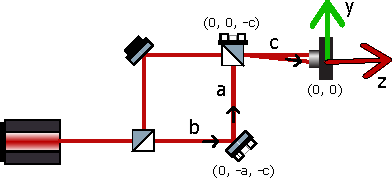
\includegraphics[width=1\linewidth]{images/MZI_matmodel.pdf}
  \begin{itemize}
    \item управление положением луча на камере $(x_0, y_0)$
    \item управление направлением $\vec{k}$
  \end{itemize}

\column{0.5\linewidth}
\begin{table} [htbp]
    \centering
    \begin{threeparttable}
        \begin{tabular}{| p{2.5cm} || p{2cm} |}
            \hline
            \hline
            параметр & значение \\
            \hline
            Mirror 2 $\to$ BS 2 & 200 mm\\
            BS 1 $\to$ Mirror 2 & 300 mm\\
            BS 2 $\to$ Camera & 100 mm\\
            radius & 0.95\\
            $\alpha_{{\mathrm{max}}(x,1)}$ & $5.2 \cdot 10^{-3}$ rad\\
            $\alpha_{{\mathrm{max}}(y,1)}$ & $3.7 \cdot 10^{-3}$ rad\\
            $\alpha_{{\mathrm{max}}(x,2)}$ & $2.6 \cdot 10^{-3}$ rad\\
            $\alpha_{{\mathrm{max}}(y,2)}$ & $1.8 \cdot 10^{-3}$ rad\\
            \hline
            \hline
        \end{tabular}
    \end{threeparttable}
\end{table}

\end{columns} 
\end{frame}


\begin{frame}
\frametitle{Видность интерференционной картины}

\begin{columns}
\column{0.4\linewidth}
\centering
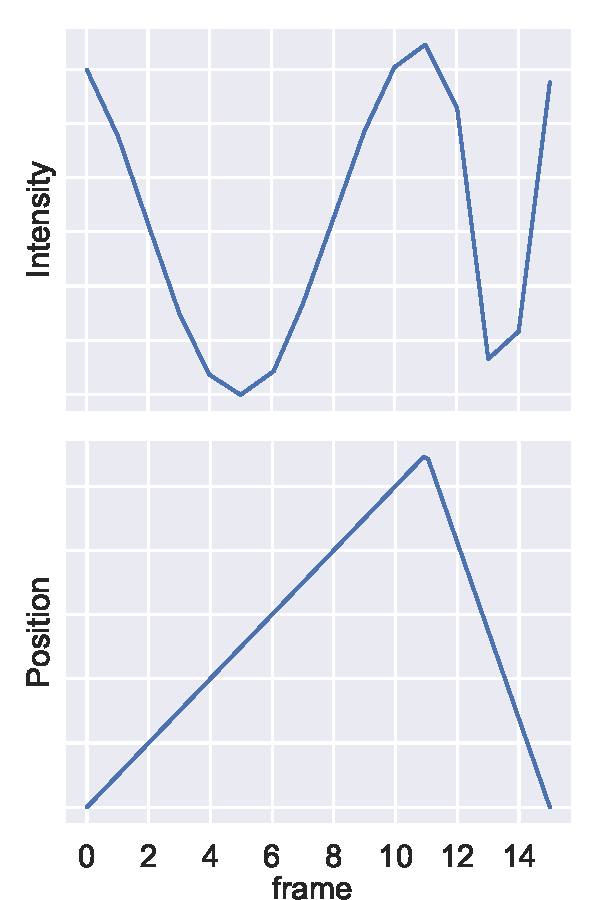
\includegraphics[width=1\linewidth]{piezo.pdf}

\column{0.5\linewidth}
\begin{align*}
& I(x,y,t)=|E_1(x,y,0)+E_2(x,y,0)e^{i\phi_{\mathrm{piezo}}(t)}|^2 \\
& I_{\mathrm{tot}}(t) = \iint_{-\infty}^{+\infty} I(x, y, t) {\mathrm{d}}x{\mathrm{d}}y \\
& V = \frac{            
        \max_{t}(I_{\mathrm{tot}}) - \min_t(I_{\mathrm{tot}})}
        {\max_{t}(I_{\mathrm{tot}}) + \min_t(I_{\mathrm{tot}})} \\
& V = \exp\left(- \frac{x_0^2 + y_0^2}{2 r^2}\right)  \exp\left[- \frac{(k_x^2 + k_y^2) r^2}{8}\right] \\
\end{align*}

\end{columns}
\end{frame}

\begin{frame}
\frametitle{Примеры интерференционных картин полученные в симуляции}
\begin{columns}
\column{0.7\linewidth}
  \centering
   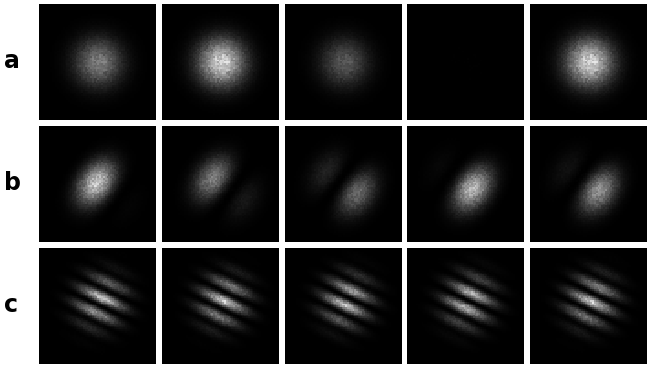
\includegraphics[scale=0.4]{images/visib_expl.png}

\column{0.5\linewidth}
\begin{description}
    \item V = 1
    \vspace{30pt}
    \item V = 0.3
    \vspace{30pt}
    \item V = 0.0026
\end{description}

\end{columns} 
\end{frame}


\begin{frame}
\frametitle{Математическая модель интерферометра Маха-Цендера с линзами}
\begin{columns}
\column{0.6\linewidth}
  \centering
   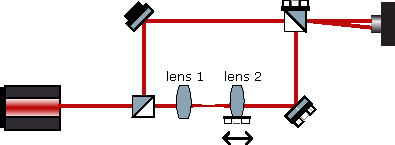
\includegraphics[width=1\linewidth]{images/MZI_expl_lenses.pdf}
  \begin{itemize}
    \item управление положением луча на камере $(x_0, y_0)$
    \item управление направлением $\vec{k}$
    \item \textcolor{red}{управление волновым фронтом}
  \end{itemize}

\column{0.5\linewidth}
\begin{table} [htbp]
    \centering
    \begin{threeparttable}
        \begin{tabular}{| p{2.5cm} || p{2cm} |}
            \hline
            \hline
            параметр & значение \\
            \hline
            BS 1 $\to$ Lens 1 & 50 mm\\
            $f_{\mathrm{lens 1}}$ = $f_{\mathrm{lens 2}}$ & 50 mm\\
            radius & 0.71 mm\\
            $\Delta_{\mathrm{max}}$ & 4.2 mm\\
            \hline
            \hline
        \end{tabular}
    \end{threeparttable}
\end{table}

\end{columns} 
\end{frame}

\begin{frame}
    \frametitle{Примеры интерференционных картин полученные на интерферометре Маха-Цендера с линзами}
    \centering
    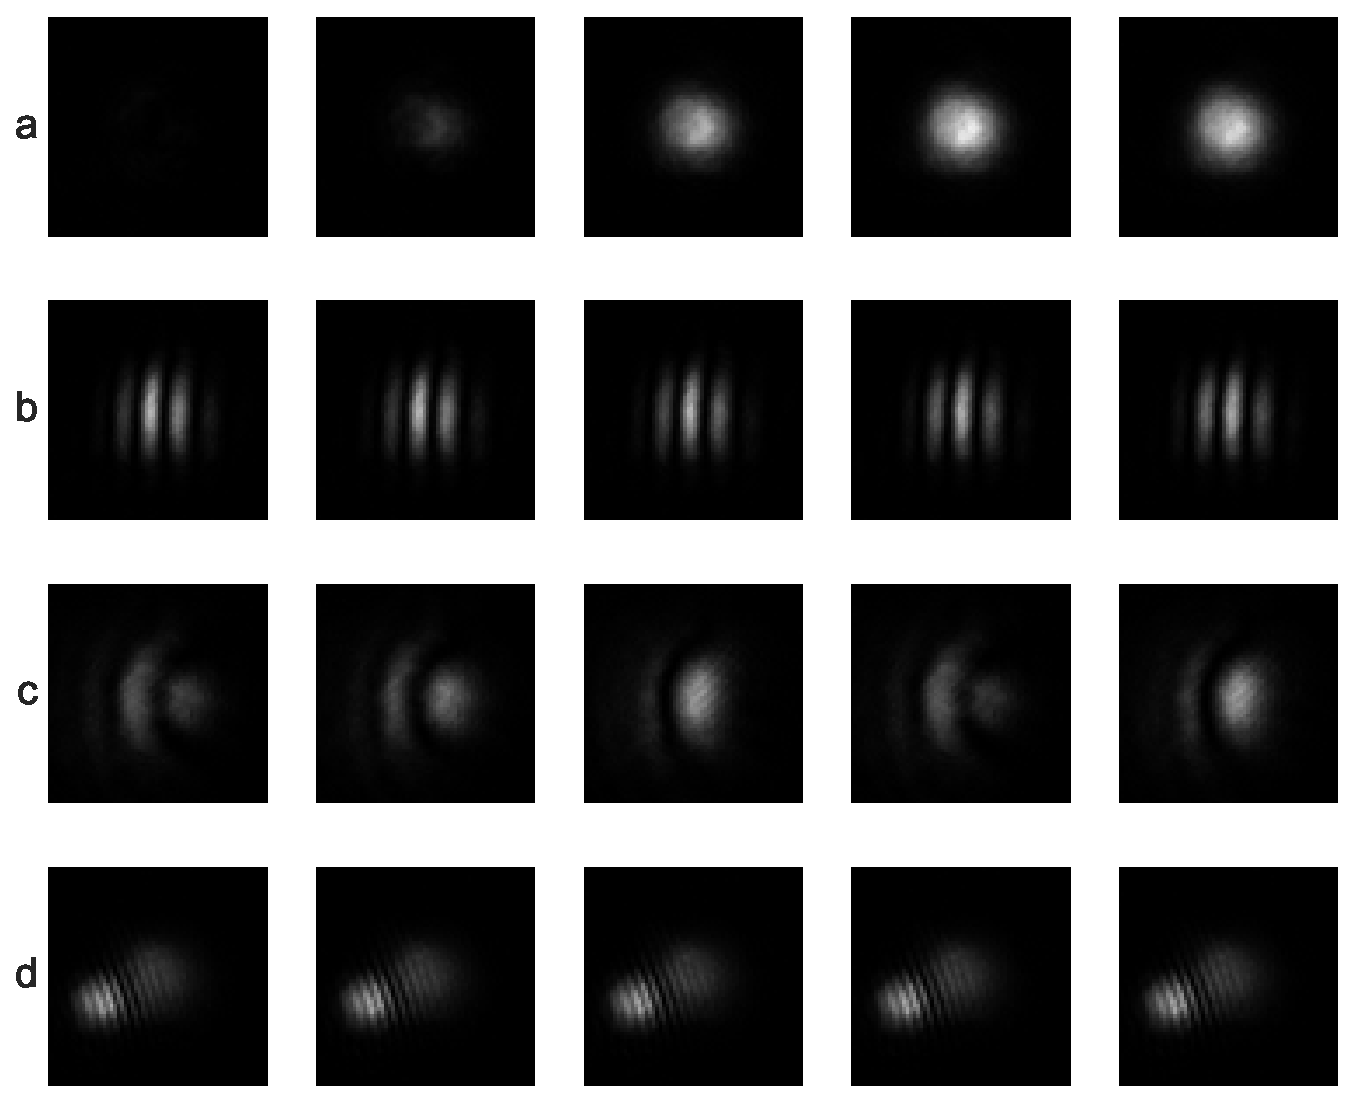
\includegraphics[width=0.8\linewidth]{images/Env_patterns.pdf}
\end{frame}

\begin{frame}
\frametitle{Видность интерференционной картины в интерферометре Маха-Цендера с линзами}
\begin{columns}
\column{0.3\linewidth}
\begin{align*}
& \dfrac{1}{q} = \dfrac{1}{\rho} - \dfrac{i \lambda}{\pi r^2} \\
& q^{\prime}=\dfrac{A q+B}{C q+D}\\
\end{align*}
\column{0.7\linewidth}
\begin{align*}
& \begin{bmatrix} A & B \\ C & D \end{bmatrix}=\begin{bmatrix} 1 & d \\ 0 & 1 \end{bmatrix} \hspace{25pt}\text{вакуум пространства длинны $d$}\\
& \begin{bmatrix} A & B \\ C & D \end{bmatrix}=\begin{bmatrix} 1 & 0 \\ -1/f & 1 \end{bmatrix} \hspace{5pt}\text{линза с фокусным расстоянием $f$} \\
& M = M_3^{ABCD} \times M_2^{ABCD} \times M_1^{ABCD}
\end{align*}
\end{columns}

\begin{equation*}
\begin{split}
    V =\frac{4}{\left(n^{2}+1\right) r_{\mathrm{u}}^{2}} \frac{1}{c} \exp \left(-\left(x_{0}^{2}+y_{0}^{2}\right)\left(\frac{1}{r_{\mathrm{u}}^{2} n^{2}}-\frac{n^{2}+1}{n^{6} r_{\mathrm{u}}^{6} c^{2}}\right)\right) \times \\ \times \exp \left(-\frac{n^{2}+1}{4 c^{2} n^{2} r_{\mathrm{u}}^{2}}\left(k_{x}^{2}+k_{y}^{2}\right)\right) \exp \left(\frac{\frac{\pi}{\lambda \rho^{\prime}}}{n^{2} r_{\mathrm{u}}^{2} c^{2}}\left(x_{0} k_{x}+y_{0} k_{y}\right)\right),
\end{split}
\end{equation*}
параметр $n=\dfrac{r_{\mathrm{l}}}{r_{\mathrm{u}}}$, $c^2 = (\dfrac{n^2 + 1}{n^2r^2_{\mathrm{u}}})^2$
\end{frame}

\begin{frame}{Численная модель интерферометра Маха-Цендера}
\begin{columns}
\column{0.5\linewidth}
\centering
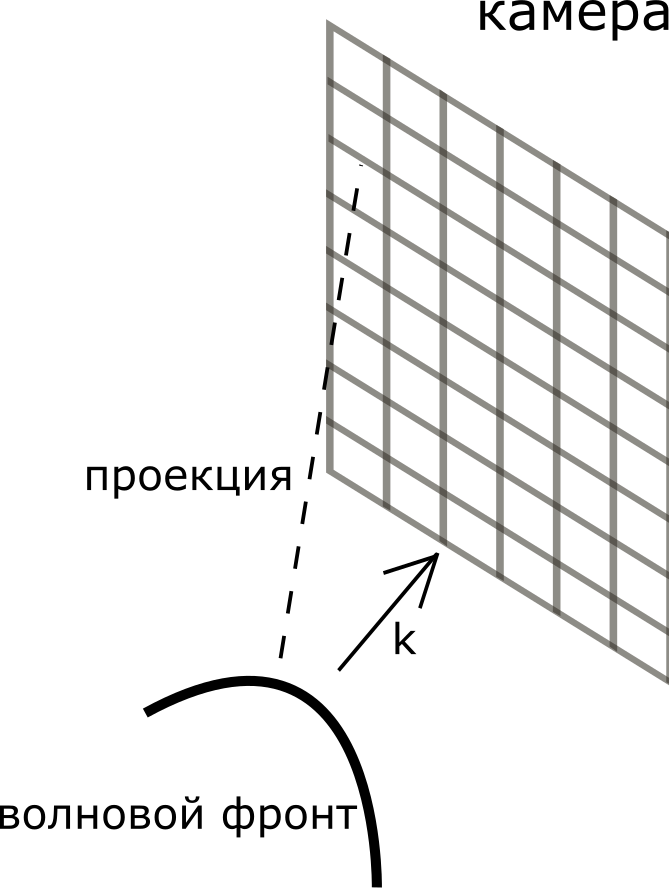
\includegraphics[width=0.8\linewidth]{images/wave_front_projection.png}
\column{0.5\linewidth}
\begin{enumerate}
    \item трассировка лучей 
    \begin{itemize}
        \item прохождение через зеркала $\vec{k}$, $(x_0, y_0)$
        \item радиус $r(z)$ и волновой фронт $\rho(z)$
    \end{itemize}
    \item вычисление интерференционной картины
    \begin{itemize}
        \item пространственное разрешение 64×64 пикселя
        \item временное разрешение 16 кадров
        \item параллельно для каждого пикселя и кадра
    \end{itemize}

    
\end{enumerate}

\end{columns}
\end{frame}

\subsection{Настройка с помощью DQN и TD3}


\begin{frame}{Настройка интерферометра с помощью алгоритма DQN}
\begin{columns}
\column{0.5\linewidth}
\centering
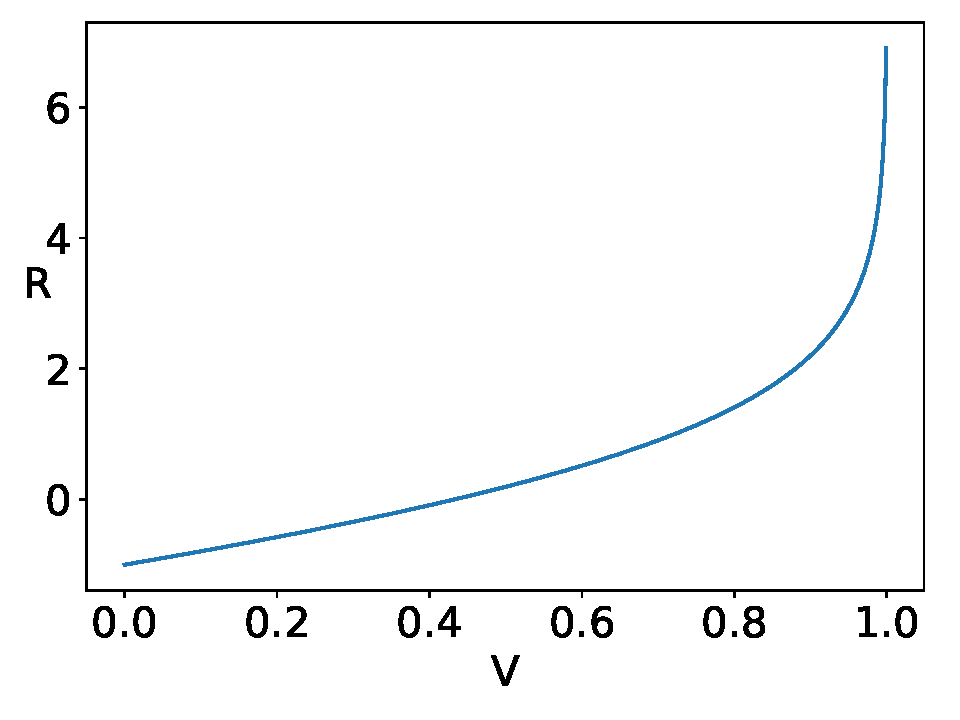
\includegraphics[width=1\linewidth]{images/reward_visib.pdf}
\column{0.5\linewidth}
\textbf{Награда}\\
$R = V - \log(1-V) - 1$\\
$V = 0.95 \to R = 2.9$\\
$V = 0.98 \to R = 3.9$\\
\textbf{Энкодер}\\
3-слойная сверточная  сеть [(32, 8, 4), (64, 4, 2), (64, 3, 1)] (Nature Mnih et.al, 2015)
\end{columns}
\vspace{10pt}
\textbf{Пространство наблюдений} 16 кадров 64x64 пикселя\\
\textbf{Пространство действий} \textcolor{red}{дискретное} (25/31) \\
\textbf{Эпизод} 100 шагов, случайный reset $\pm \alpha_{\mathrm{max}}$, $\pm \Delta_{\mathrm{max}}$\\
\textbf{Параметры} $\gamma = 0.99 \to  \Delta = \frac{1}{1 - \gamma} = \textcolor{red}{100}$, total steps $10^8$, buffer size $10^6$, batch size $32$\\

\end{frame}

\begin{frame}{Настройка интерферометра с помощью алгоритма TD3}
\begin{columns}
\column{0.5\linewidth}
\centering
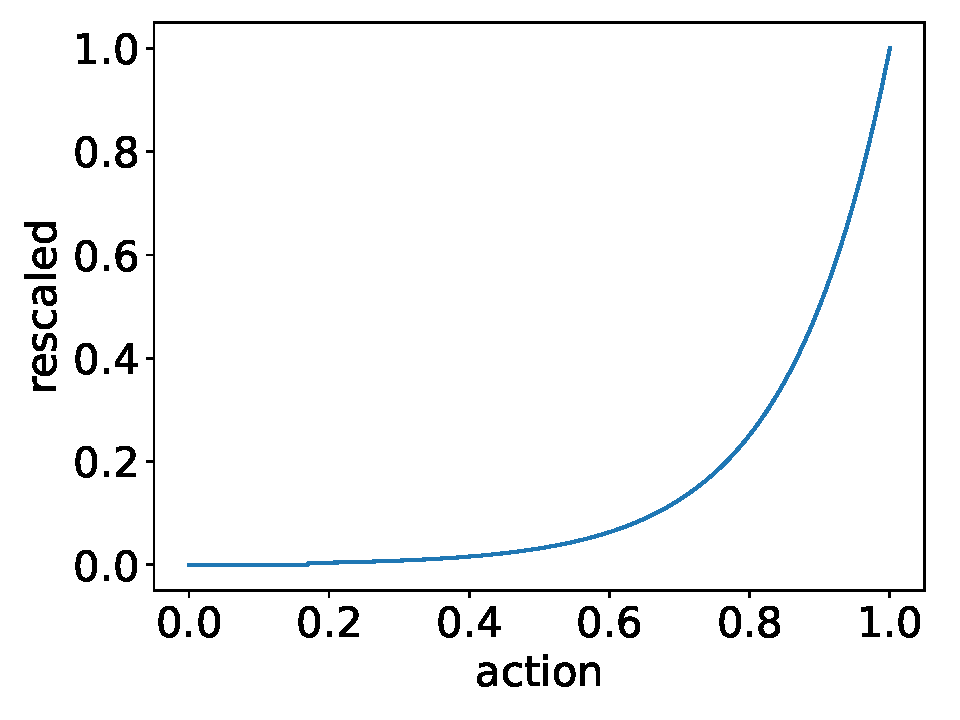
\includegraphics[width=1\linewidth]{images/rescale.pdf}
\column{0.5\linewidth}
\textbf{Награда}\\
$R = V - \log(1-V)$\\
\textbf{Масштабирование действий}\\
\vspace{-15pt}
\begin{equation*}
a^{\prime} =
   \begin{cases}
    {\mathrm{sign}}(a) \cdot 1000^{|a| - 1}, |a_0| > 0.17
    \\
    0
  \end{cases}
\end{equation*}
\textbf{Энкодер}\\
VGG-16
\end{columns}
\vspace{10pt}
\textbf{Пространство действий} \textcolor{red}{непрерывное} ($\mathcal{R}^4$/$\mathcal{R}^5$)\\
\textbf{Параметры} $\gamma = 0.8 \to  \Delta = \frac{1}{1 - \gamma} = \textcolor{red}{5}$, total steps $10^6$, buffer size $10^5$, batch size $32$ \\

\end{frame}

\subsection{Программно-аппаратный комплекс Интерферобот}

\begin{frame}{Программно-аппаратный комплекс Интерферобот}
\begin{columns}
\column{0.35\linewidth}
\centering
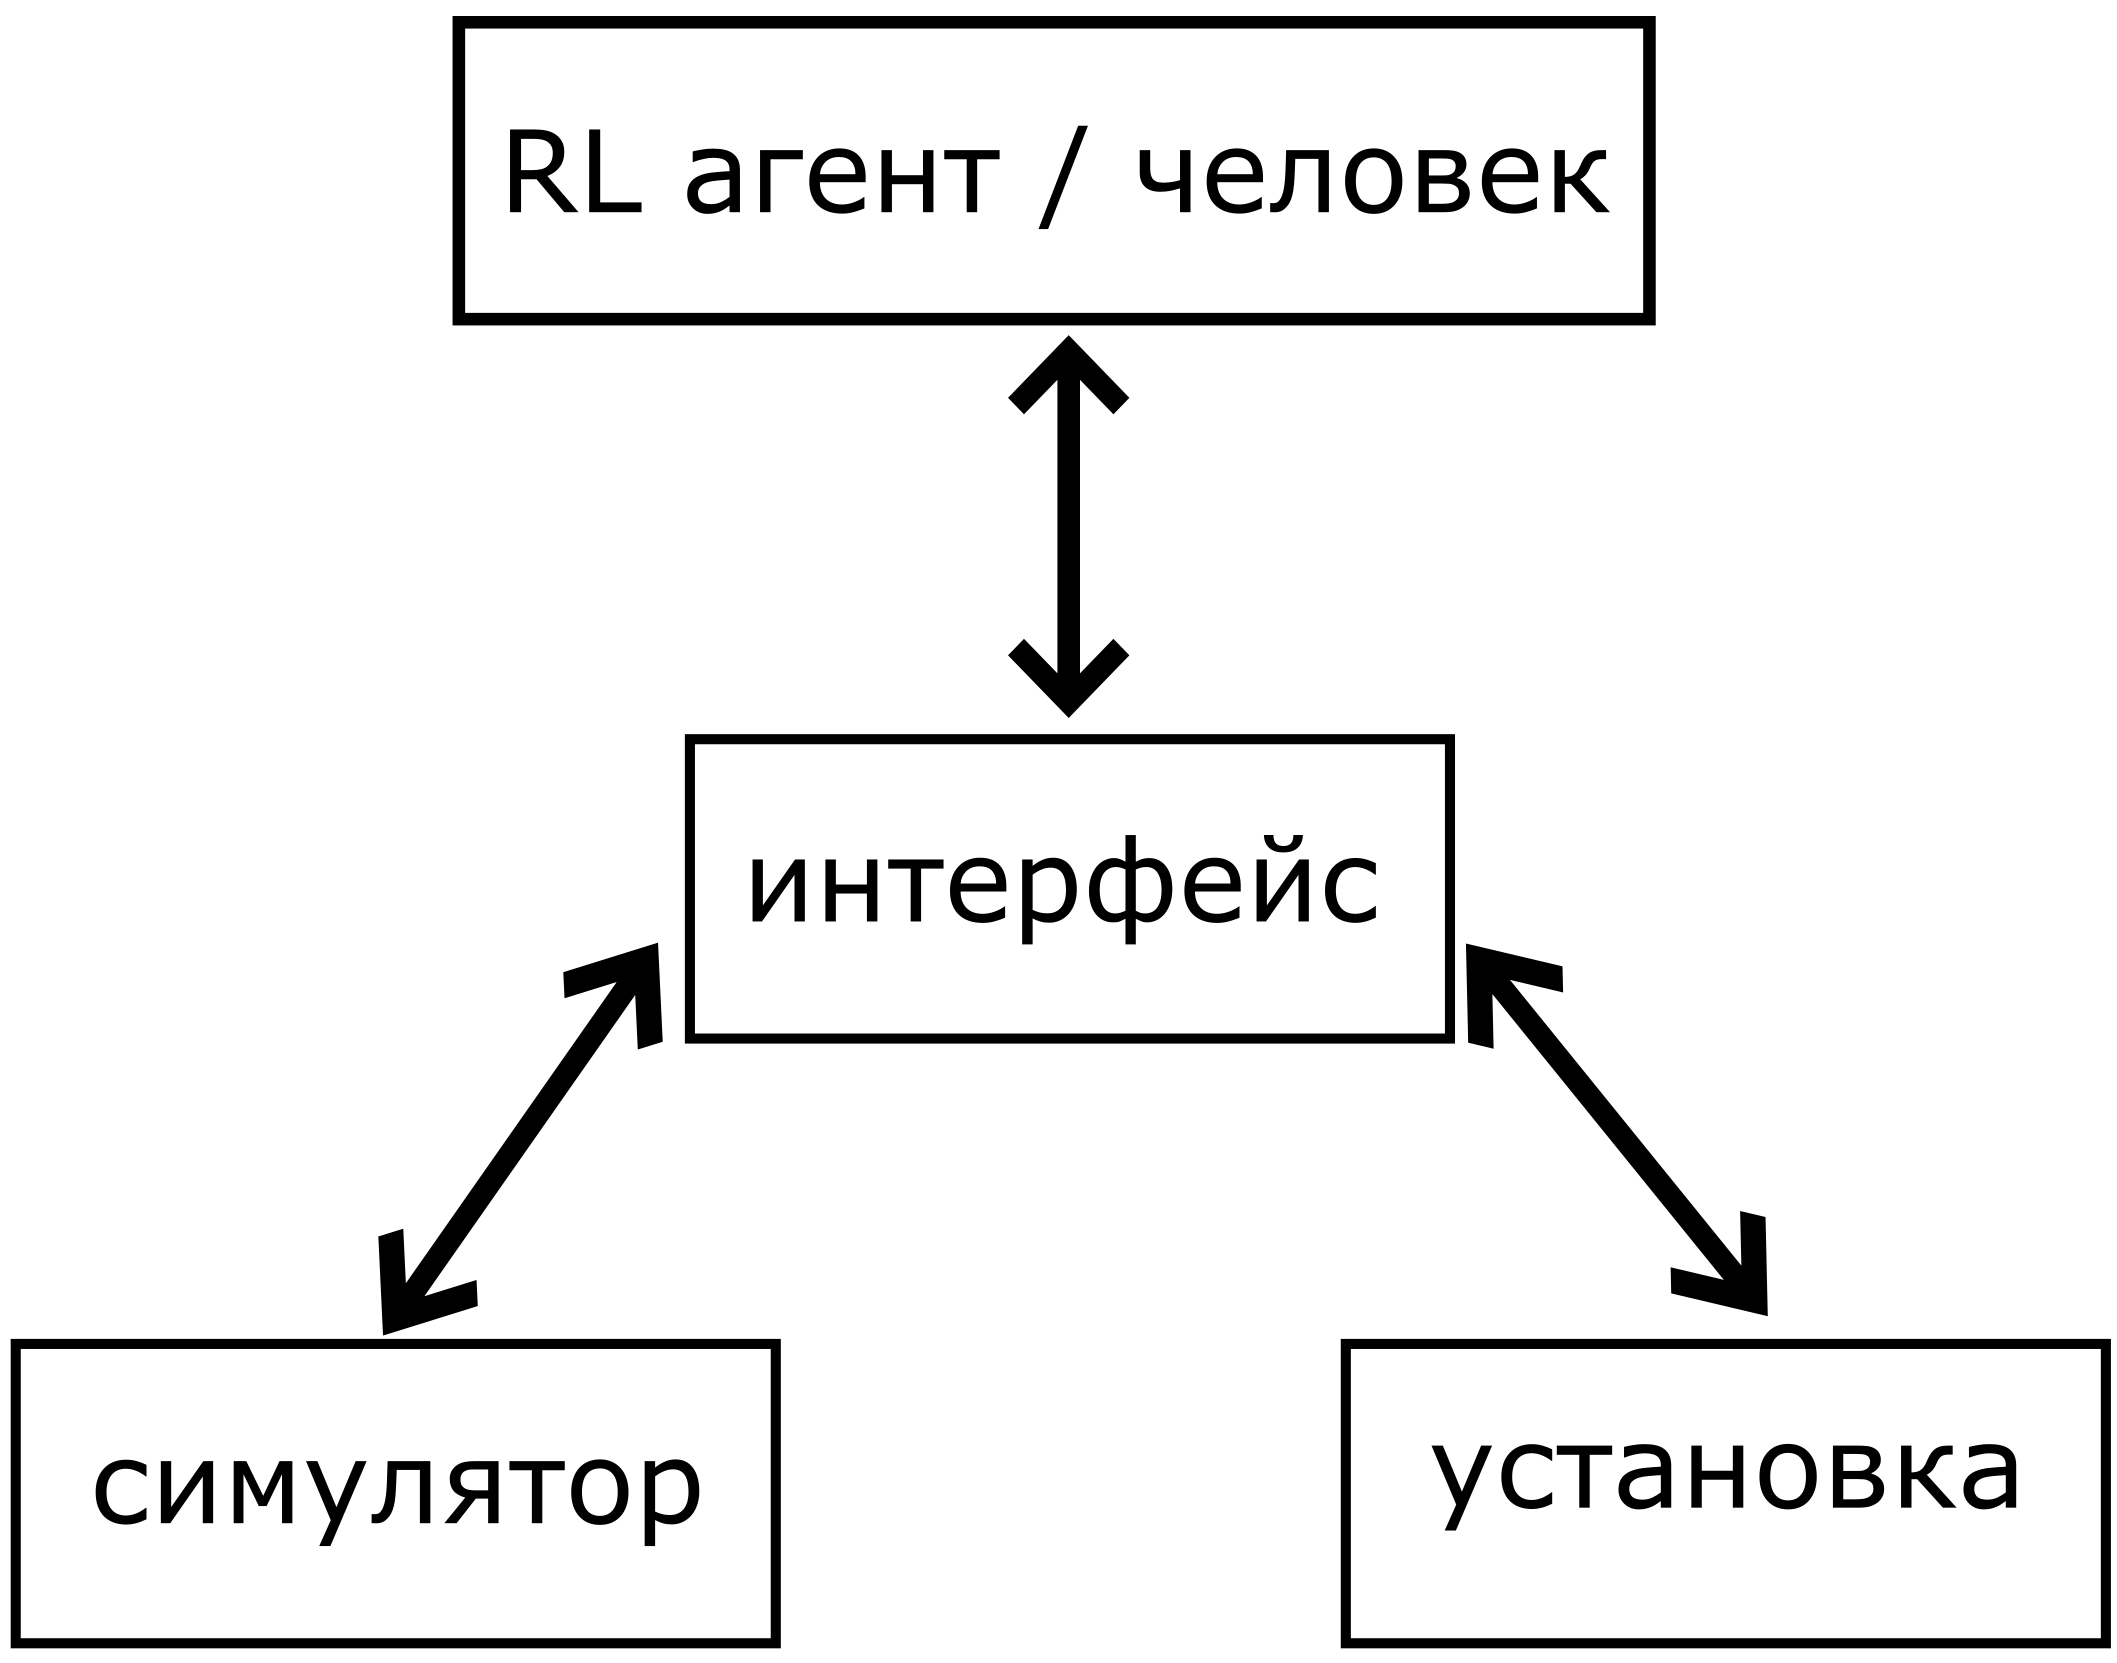
\includegraphics[width=1\linewidth]{images/interferobot_complex.png}
Схема взаимодействия модулей
\column{0.65\linewidth}
\centering
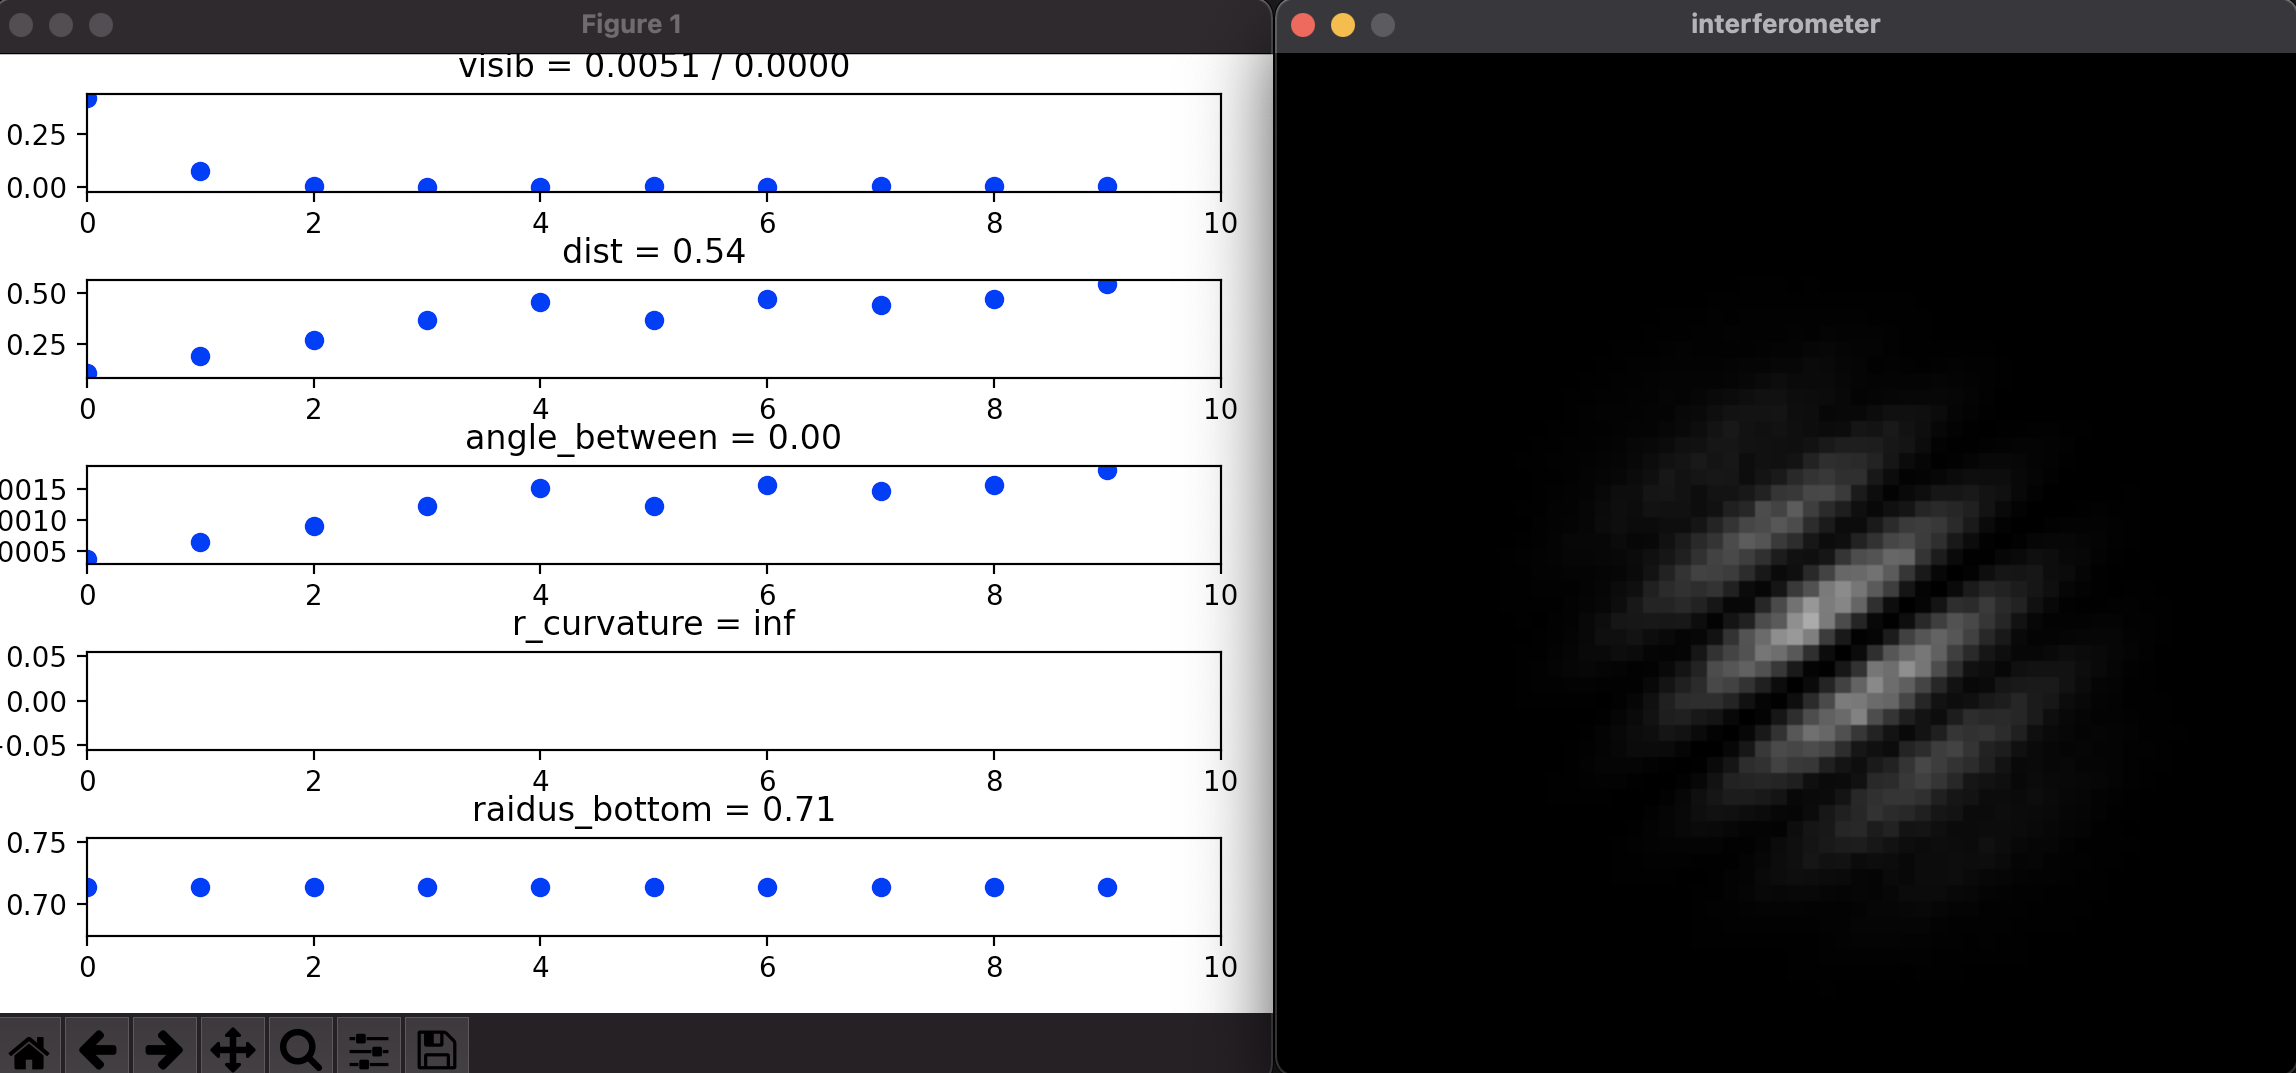
\includegraphics[width=1\linewidth]{images/gui.png}
Графический интерфейс пользователя
\end{columns}
\vspace{15pt}
C++, Python3\\
200 состояний среды (16x64х64) за одну секунду (16 потоков на intel core i7)
\end{frame}

\begin{frame}{Перенос из симуляции в реальность}
\begin{columns}
\column{0.4\linewidth}
\centering
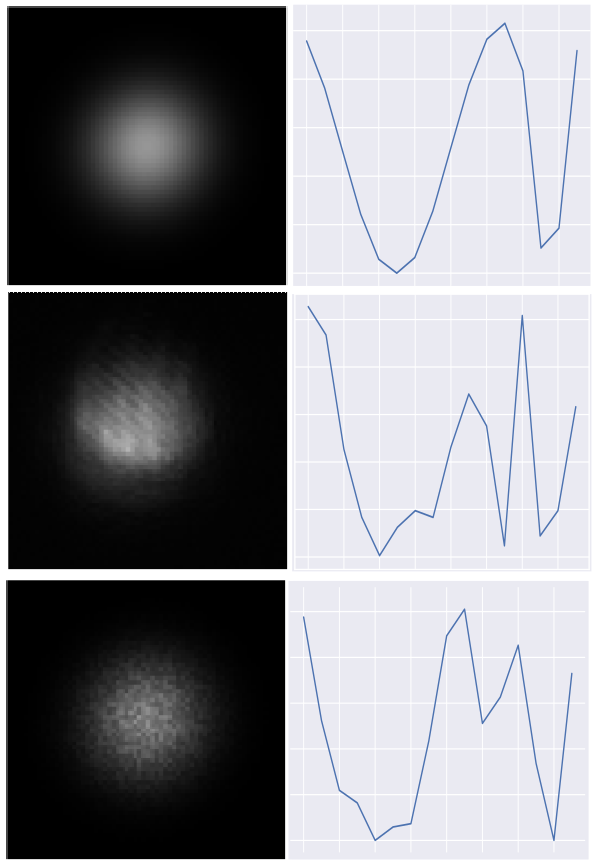
\includegraphics[width=1\linewidth]{beamsamples.png}
\column{0.6\linewidth}
\textbf{в начале каждого эпизода}
\begin{itemize}
    \item radius randomization $\pm 20\%$
\end{itemize}
\textbf{на каждом шаге}
\begin{itemize}
    \item exposure randomization $\pm 30\%$
    \item image noise $20\%$
    \item cycle frame shift
    \item duty cycle randomization
    \item phase noise $\phi \sim \mathcal{N}(\frac{2\pi k}{N}, 0.5)$
\end{itemize}
\end{columns}
\end{frame}

\begin{frame}[allowframebreaks]{Настройка интерферометра Маха-Цендера без линз}
\begin{columns}
\column{0.5\linewidth}
\centering
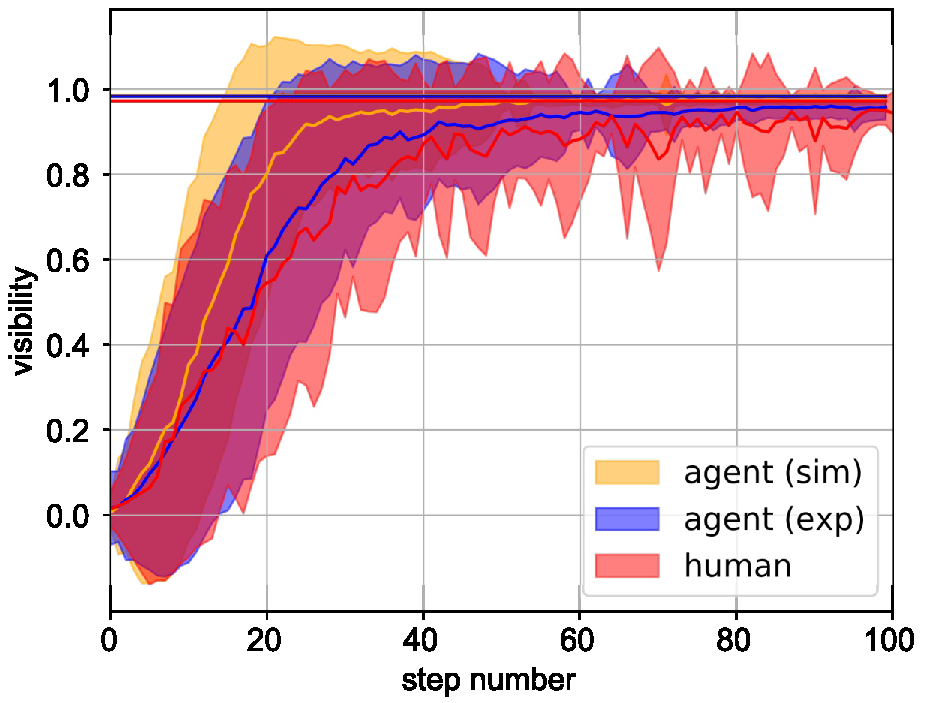
\includegraphics[width=1\linewidth]{images/eval1_visib_step.pdf}
\column{0.5\linewidth}
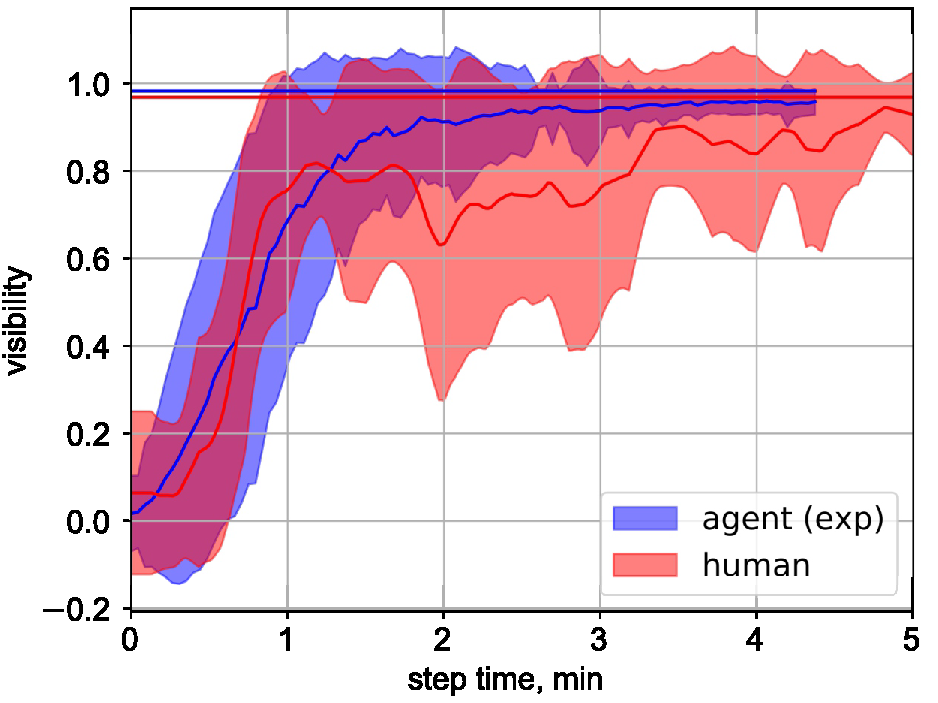
\includegraphics[width=1\linewidth]{images/eval1_visib_time.pdf}
\end{columns}

\begin{table} [htbp]
    \centering
    \begin{threeparttable}
        \caption*{Средняя наибольшая видность достигнутая при настройке}
        \begin{tabular}{| p{3cm} || p{3cm} || p{3cm} |}
            \hline
            \hline
            DQN (sim) & DQN (exp) & Human \\
            \hline
            0.986 & 0.983 & 0.972 \\
            \hline
            \hline
        \end{tabular}
    \end{threeparttable}
\end{table}
\framebreak
\begin{minipage}{\textwidth}
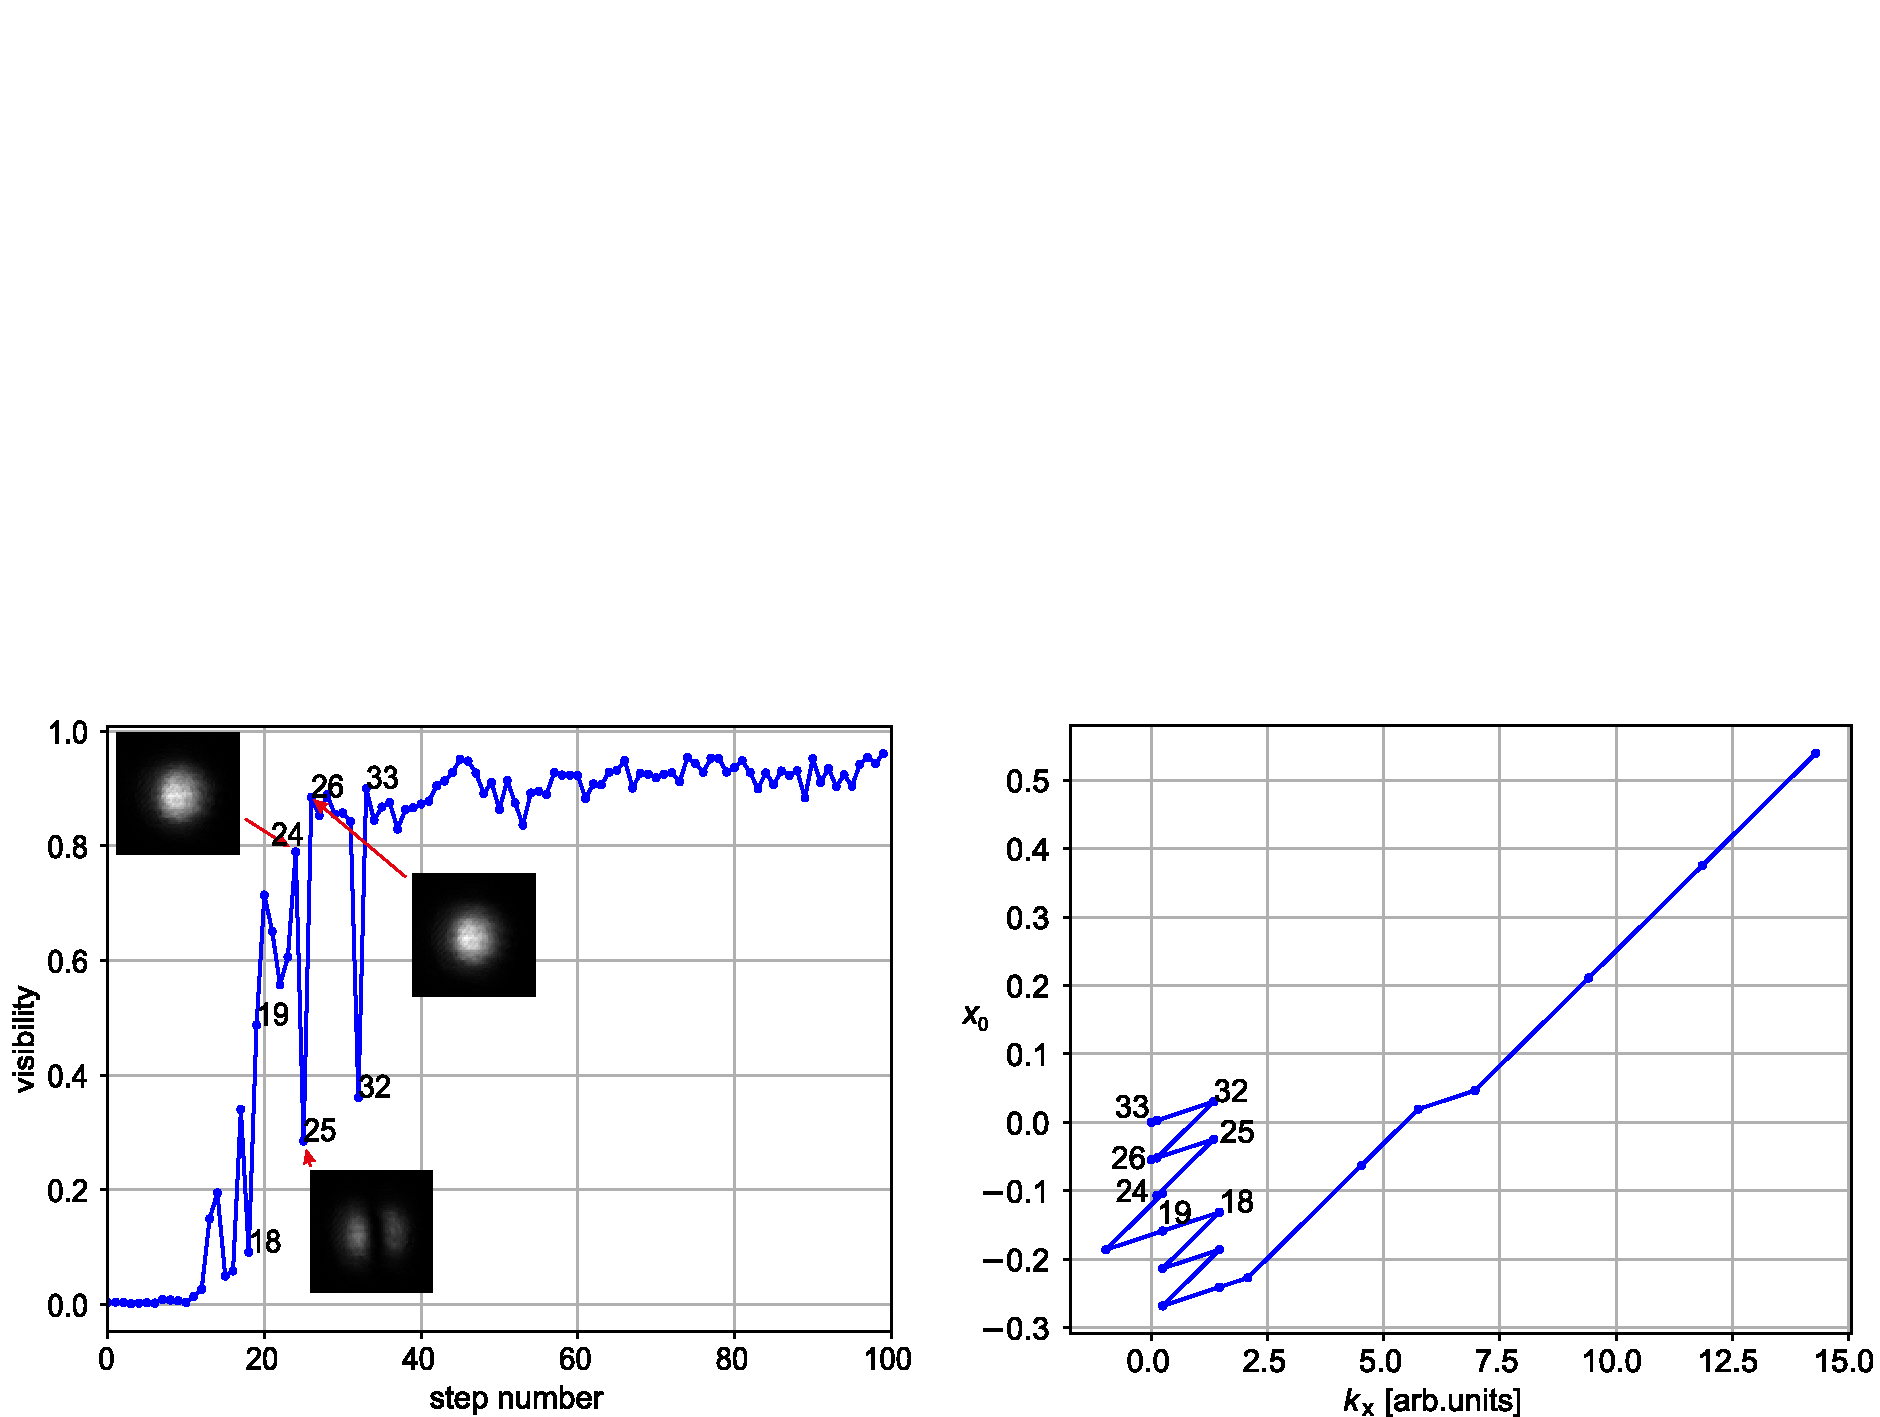
\includegraphics[width=1\linewidth]{DQN_analysis.pdf}
\end{minipage}
\begin{minipage}{\textwidth}
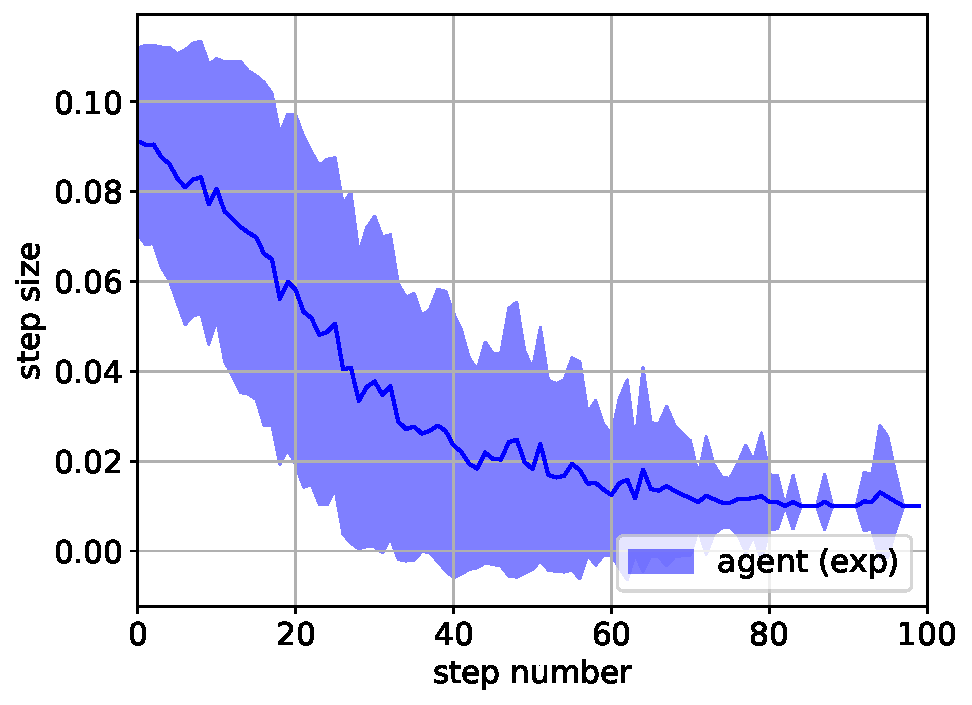
\includegraphics[width=0.5\linewidth]{images/agent_step_size.pdf}
\end{minipage}

\framebreak 

\begin{table} [htbp]
    \centering
    \begin{threeparttable}
        \caption*{Анализ влияния шумов используемых при обучении агента на качество настройки физической установки}
        \begin{tabular}{| p{5cm} || p{2cm} || p{2cm} |}
            \hline
            \hline
             & visibility & return \\
            \hline
            All randomizations  & $\textbf{0.96} \pm \textbf{0.02}$ & $\textbf{221} \pm \textbf{54}$ \\
            No radius randomization & $0.74 \pm 0.20$ & $85 \pm 69$ \\
            No exposure randomization& $0.91 \pm 0.04$ & $178 \pm 39$ \\
            No image noise & $0.82 \pm 0.07$ & $129 \pm 43$ \\
            No duty cycle and frame shift  &  $0.89 \pm 0.07$ & $200 \pm 42$ \\
            \hline
            \hline
        \end{tabular}
    \end{threeparttable}
\end{table}
\end{frame}

\begin{frame}[allowframebreaks]{Настройка интерферометра Маха-Цендера с системой линз}
\begin{columns}
\column{0.5\linewidth}
\centering
\includegraphics[width=1\linewidth]{images/DQN_vs_TD3.pdf}
\column{0.5\linewidth}
\centering
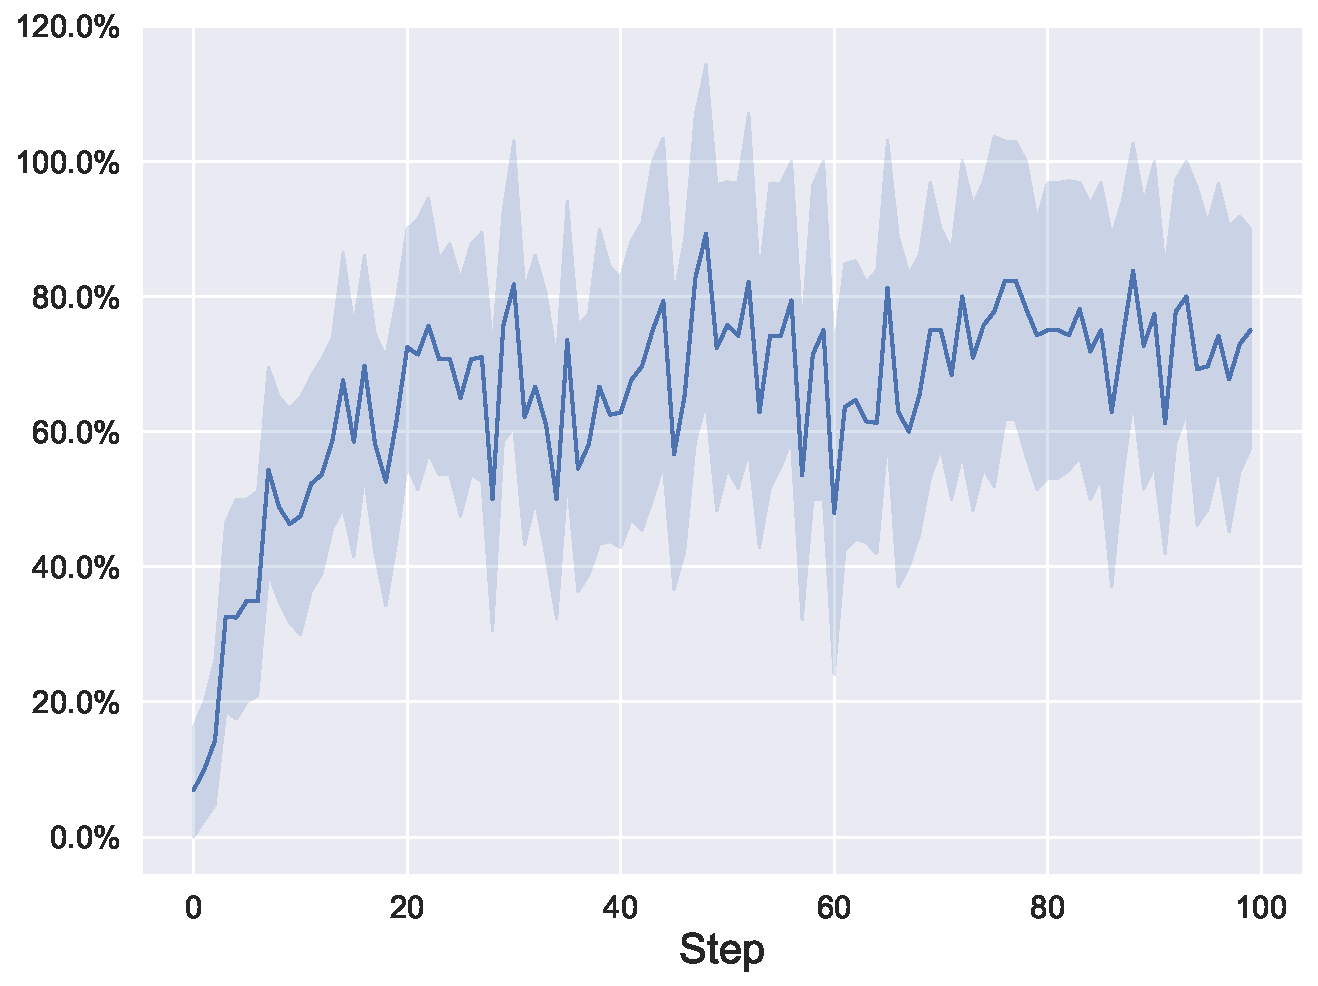
\includegraphics[width=1\linewidth]{images/parallel_actions_count_for_each_axis.pdf}
\end{columns}
\begin{table} [htbp]
    \centering
    \begin{threeparttable}
        \begin{tabular}{| p{2cm} || p{2cm} || p{2cm} || p{3cm} |}
            \hline
            \hline
            &V $\ge 0.92$ & V $\ge 0.95$ & V $\ge 0.98$ \\
            \hline
            Human &  93.9 (\textbf{0\%})  & 103.6 (\textbf{0\%}) & 129.6 (10\%)\\
            TD3 &  \textbf{56.16} (\textbf{0\%}) & \textbf{75.06} (\textbf{0\%}) & \textbf{120.1} (\textbf{4\%})\\
            DQN &  98.7 (7.6\%) & 116.1 (7.6\%) & 156.4 (10.6\%)\\
            \hline
            \hline
        \end{tabular}
    \end{threeparttable}
\end{table}

\framebreak 

\begin{columns}
\column{0.5\linewidth}
\centering
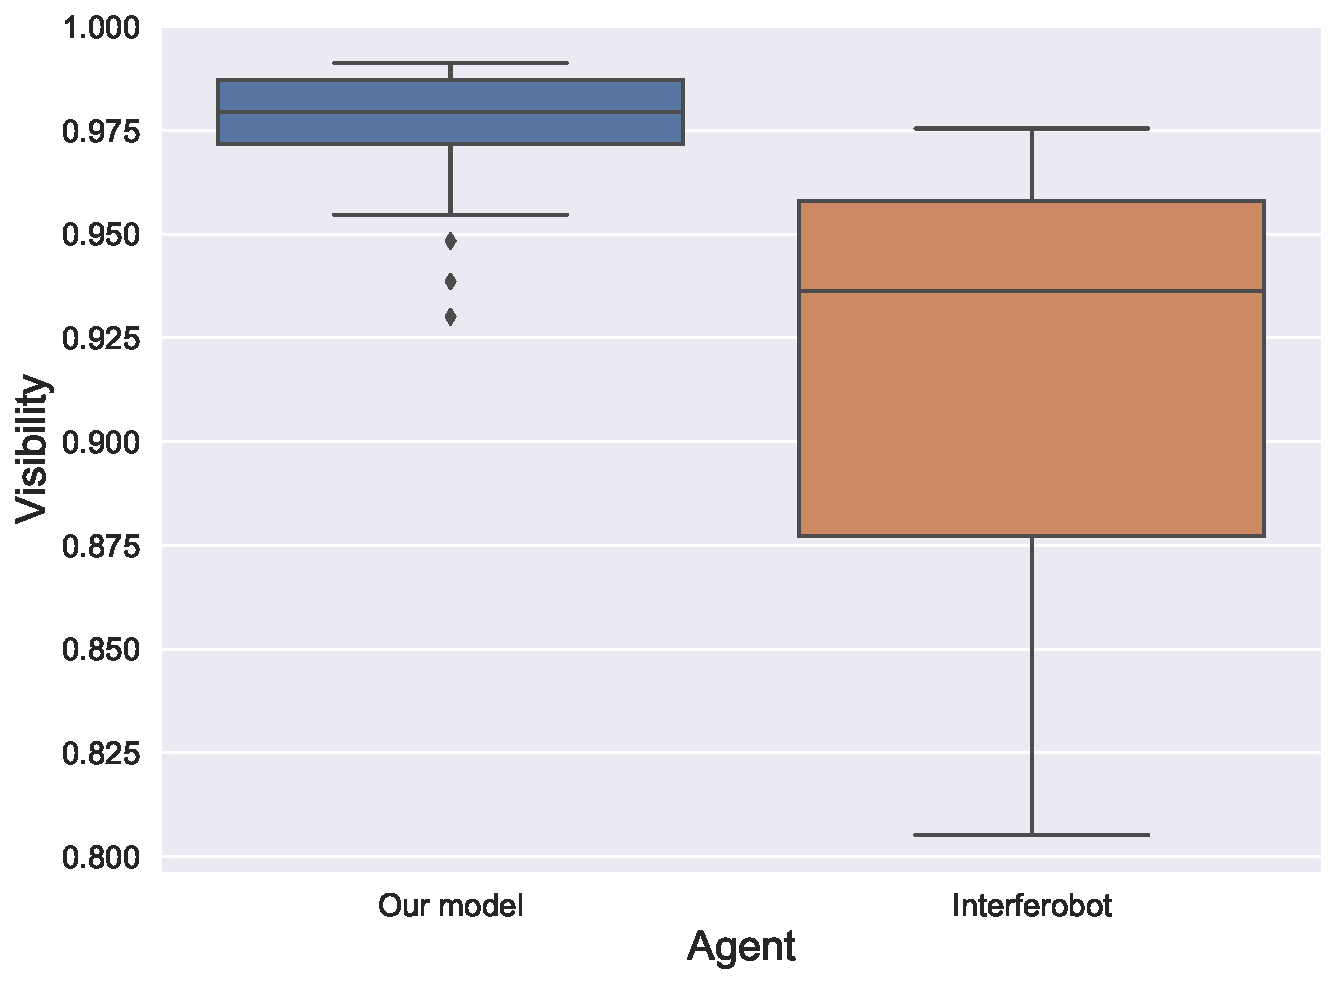
\includegraphics[width=1\linewidth]{images/DQN_vs_TD3_box.pdf}
Межквантильный размах видности
\column{0.5\linewidth}
\centering
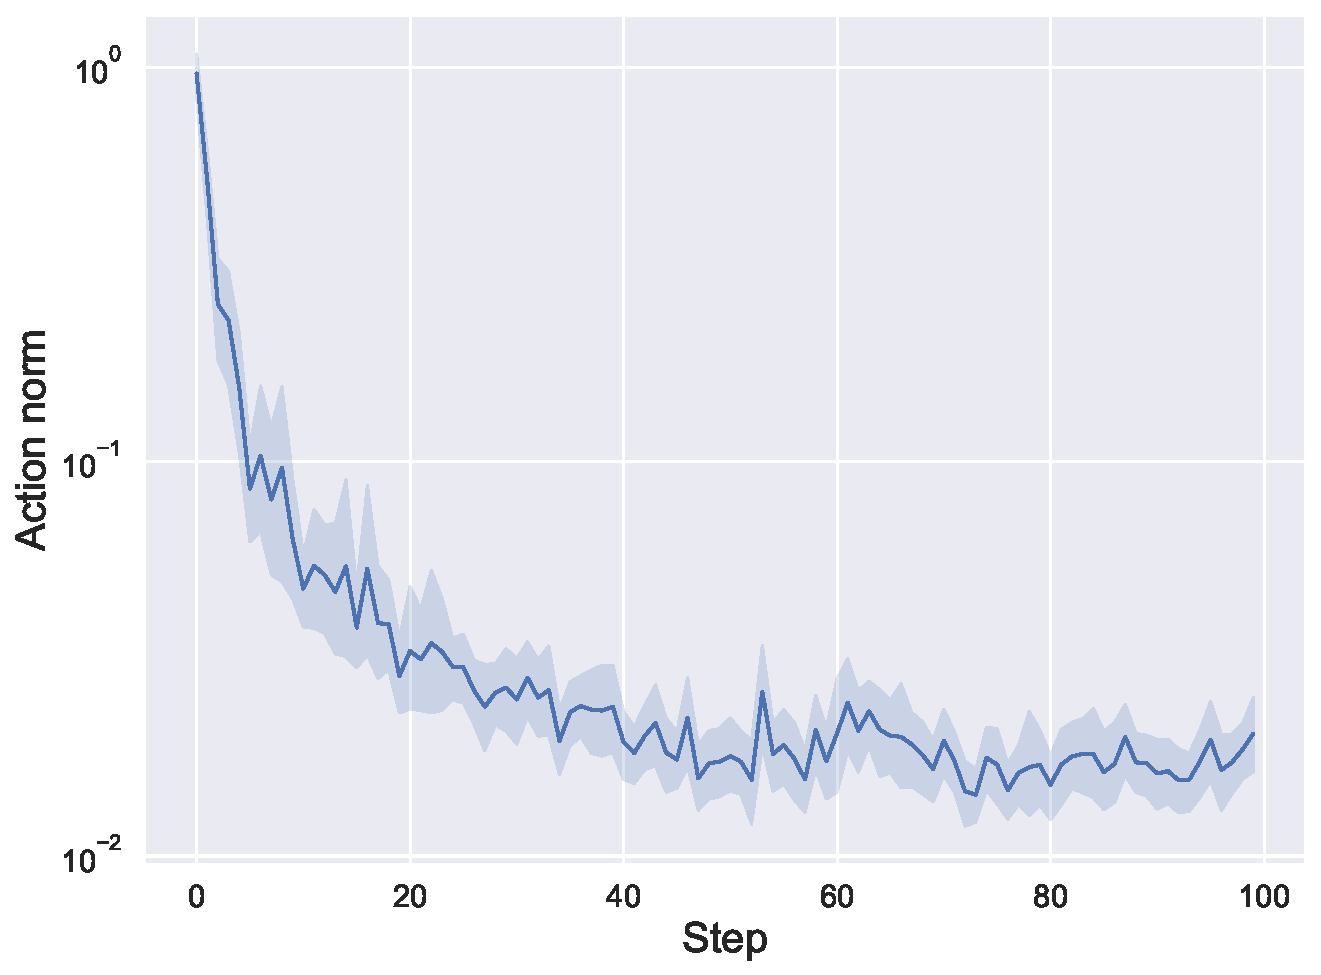
\includegraphics[width=1\linewidth]{images/action_norm_decrease.pdf}
Средняя амплитуда действий
\end{columns}

\framebreak

\begin{table} [htbp]
    \centering
    \begin{threeparttable}
        \caption*{Анализ эффективности фазового шума и масштабирования действий. PN: фазовый шум; AR: масштабирование действий.}
        \begin{tabular}{| p{3cm} || p{3cm} || p{3cm} |}
            \hline
            \hline
            агент & средняя видность за последние 40 шагов & стандартное отклонение \\
            \hline
            TD3 + AR + PN & \textbf{0.98} & \textbf{0.03} \\
            TD3 + AR & 0.95 & 0.06\\
            DQN + PN & 0.90 & 0.08\\
            TD3& 0.83 & 0.18\\
            \hline
            \hline
        \end{tabular}
    \end{threeparttable}
\end{table}

\end{frame}


\begin{frame}{Выводы}
\begin{itemize}
    \item Разработан симулятор интерферометра Маха-Цендера
    \item Интерферометр может быть успешно настроен методами RL
    \item Разработан программно-аппаратный комплекс Интерферобот
    \item Предложен набор шумов и функция награды
    \item Реализовано два подхода к представлению пространства действий дискретный (DQN агент) и непрерывный (TD3 агент)
    \item  Качество работы TD3 агента превосходит качество настройки эксперта

\end{itemize}
    



\end{frame}

% \subsection{Не нумерованные}

\section{Разработка алгоритма для игры NetHack с
применением машинного обучения с подкреплением}

\subsection{Декомпозиция игры NetHack на подзадачи}

\begin{frame}
\frametitle{NetHack challenge}
\begin{columns}
\column{0.6\linewidth}
  \centering
  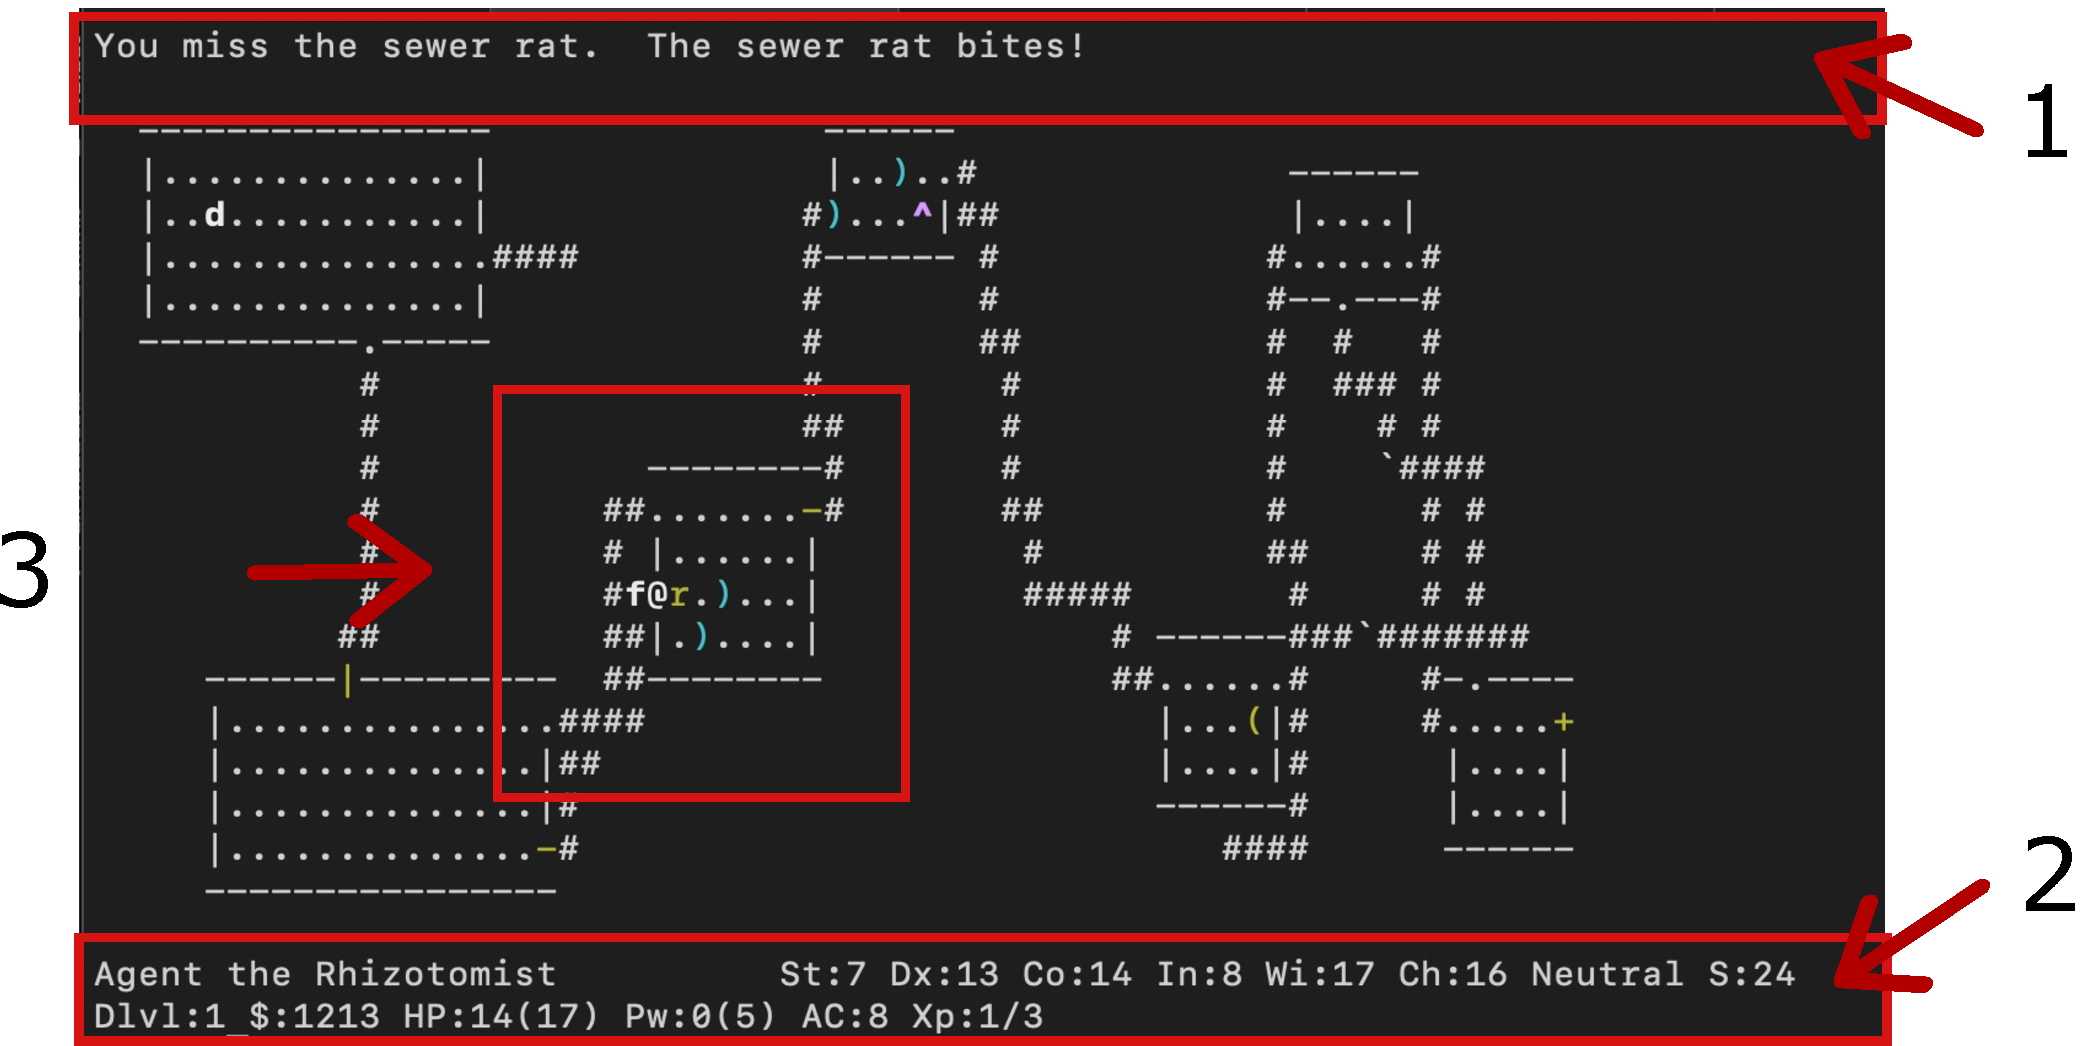
\includegraphics[width=1\linewidth]{images/nethack_map_view.pdf}
\column{0.55\linewidth}
\begin{enumerate}
    \item текстовое сообщение описывающее текущее событие
    \item статистика агента (здоровье, золото, сила, и др.) 
    \item окно центрированное возле текущего положения агента (@).
\end{enumerate}
\end{columns} 
\vspace{20pt}
В чем ``challange''?
\begin{itemize}
    \item Процедурная генерация среды
    \item NetHack – очень длинная игра
    \item Много модальные наблюдения
    \item Сложное пространство действий
\end{itemize}


\end{frame}


\begin{frame}{Декомпозиция игры NetHack на подзадачи}
\begin{columns}
\column{0.5\linewidth}
\centering
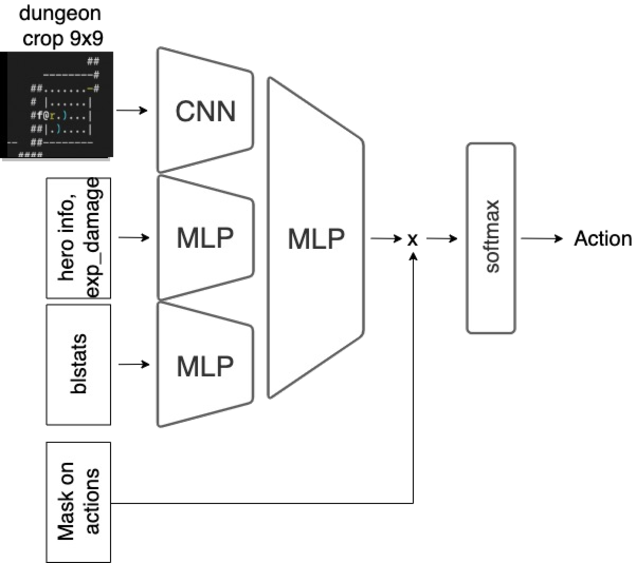
\includegraphics[width=1\linewidth]{images/raph_arch.pdf}
\column{0.5\linewidth}
\textbf{Пространство действий}. 
\begin{itemize}
    \item шаг или ближняя атака (x8 направлений)
    \item дальняя атака (x8 направлений)
    \item пропуск хода
    \item заклинание Elbereth
    \item молитва
\end{itemize}
\textbf{Передача управления}. 
$distance(agent, monster) < 5$
\end{columns}
\end{frame}

\subsection{Объединение RL и алгоритмического подхода}

\begin{frame}
\frametitle{Обучение иерархического агента совмещающего обучение с подкреплением и алгоритмический подход}
\begin{columns}
\column{0.7\linewidth}
\centering
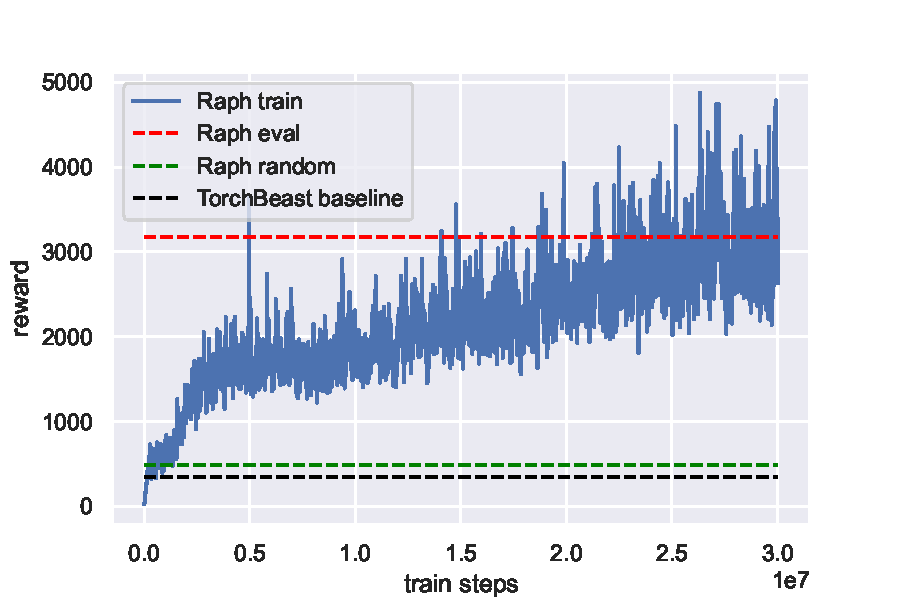
\includegraphics[width=1\linewidth]{images/raph_train.pdf}
\column{0.5\linewidth}
\begin{itemize}
    \item ближняя атака 66\%
    \item дальняя атака 21.6\%
    \item пропуск хода 11\%
    \item ``Elbereth'' 0.3\%
    \item молитва 0.1\%
\end{itemize}
\end{columns}
\end{frame}


\begin{frame}{Выводы}
\begin{itemize}
    \item Разработан гибридный нейро-символьный агент для среды NetHack
    \item RL агент решает одну из наиболее сложных задач возникающих в среде NetHack — сражение с монстрами.
    \item В соревновании по игре NetHack (NeurIPS 2021 Competition Track) агент занял \textcolor{red}{первое место}
\end{itemize}
    
\end{frame}

%\begin{frame}
%    \frametitle{Изображения по-вертикали}
%    \centering
%    \vfill
%    \includegraphics[width=0.8\linewidth,height=0.1\textheight]{latex%} \\
%    \TeX
%    \vfill
%    \includegraphics[width=0.8\linewidth,height=0.2\textheight]{latex%} \\
%    \LaTeX
%    \vfill
%    \includegraphics[scale=0.2]{latex} \\
%    \vfill
%\end{frame}


%\begin{frame}
%    \frametitle{Изображения по-горизонтали}
%    \begin{minipage}[t]{0.47\linewidth}
%        \textbf{Составная \\ подпись 1}
%        \center{\includegraphics[width=1\linewidth]{knuth1}}
%    \end{minipage}
%    \hfill
%    \begin{minipage}[t]{0.47\linewidth}
%        \textbf{Составная \\ подпись 2}
%        \center{\includegraphics[width=1\linewidth]{knuth2}}
%    \end{minipage}
%\end{frame}


%\begin{frame}
%    \frametitle{Разделяющие линии}
%    \begin{minipage}[c]{0.47\linewidth}
%        \center{\includegraphics[width=1\linewidth]{latex}}
%        \bigskip
%        \hrule{}
%        \bigskip
%        \textbf{Составная \\ подпись 1}
%    \end{minipage}
%    \hfill
%    \vrule{}
%    \hfill
%    \begin{minipage}[c]{0.47\linewidth}
%        \flushright
%        \textbf{Составная \\ подпись 2}
%        \center{\includegraphics[width=1\linewidth]{knuth2}}
%    \end{minipage}
%\end{frame}

\section{Метод управления линейной и угловой скоростью шагающего робота основанный на обучении с подкреплением}

\begin{frame}{Постановка задачи управления шагающим роботом}
\begin{columns}
\column{0.5\linewidth}
\centering
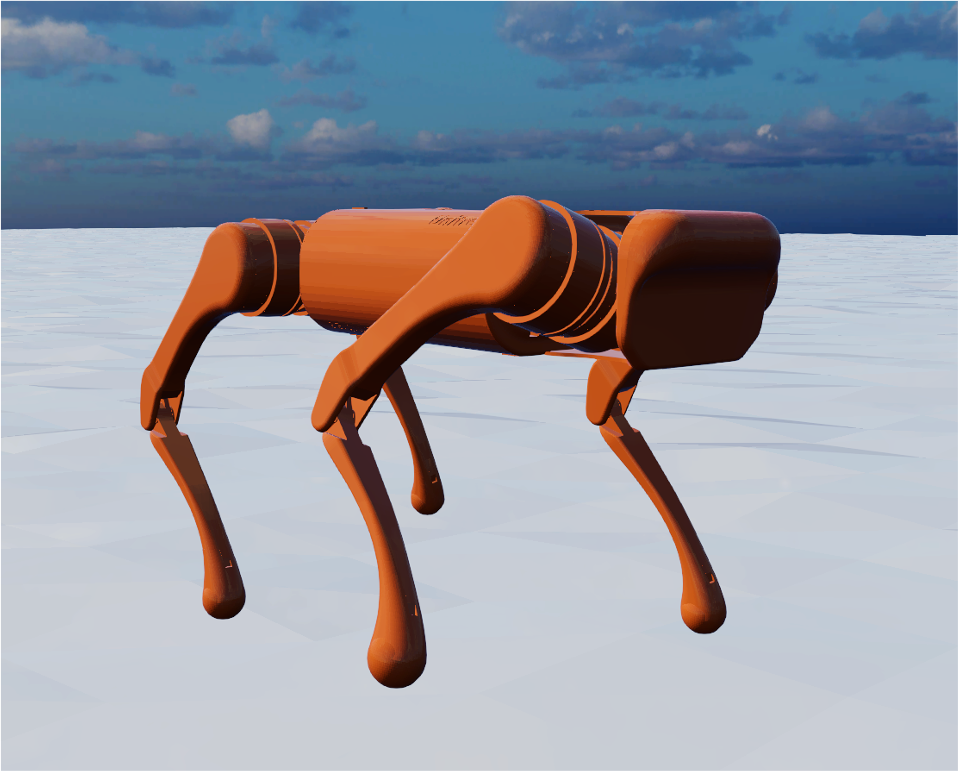
\includegraphics[width=1\linewidth]{unitree_a1.png}
\column{0.5\linewidth}
\begin{itemize}
    \item ``Движение вперед / назад''
	\item ``Движение вперед с заданной скоростью''
    \item ``Поворот по / против часовой стрелке''
\end{itemize}
\end{columns}
\textbf{Пространство наблюдений} положение корпуса, суставов, линейные и угловые скорости ($\mathcal{R}^{50}$) 
\\
\textbf{Пространство действий} целевые положения суставов ($\mathcal{R}^{12}$ )

\end{frame}

\begin{frame}{Метод управления линейной и угловой скоростью шагающего робота основанный на обучении с подкреплением}
\begin{multline*}
    r = k_{torso\ height} \cdot r_{torso\ height} +
    k_{torque} \cdot r_{torque} +\\
    k_{joint\ speed} \cdot r_{joint\ speed} +
    k_{slip} \cdot r_{slip} +\\
    k_{work} \cdot r_{work} + 
    k_{ground\ impact} \cdot r_{ground\ impact} +\\
    k_{z\ acceleration} \cdot r_{z\ acceleration} +  k_{velocity} \cdot r_{velocity} +\\
    k_{transverse\ and\ rotation} \cdot r_{transverse\ and\ rotation}
\label{eq:unitree_reward}
\end{multline*}

\begin{align*}
& r_{velocity} = \mathrm{clip}(V_x \cdot D / \hat{V_x}, 0, 1) \hspace{18pt}\text{``Движение вперед / назад''}\\
& r_{velocity} = \max(1 - |V_x / \hat{V_x} - 1|, 0) \hspace{1pt}\text{``Движение вперед с заданной скоростью''}\\
& r_{velocity} = \mathrm{clip}(W_z \cdot D / \hat{W_z}, 0, 1) \hspace{13pt}\text{``Поворот по / против часовой стрелки''}
\end{align*}
\end{frame}

\begin{frame}{Оценка результатов работы в симуляции}
\begin{figure}[h]
\begin{subfigure}{.5\textwidth}
  \centering
  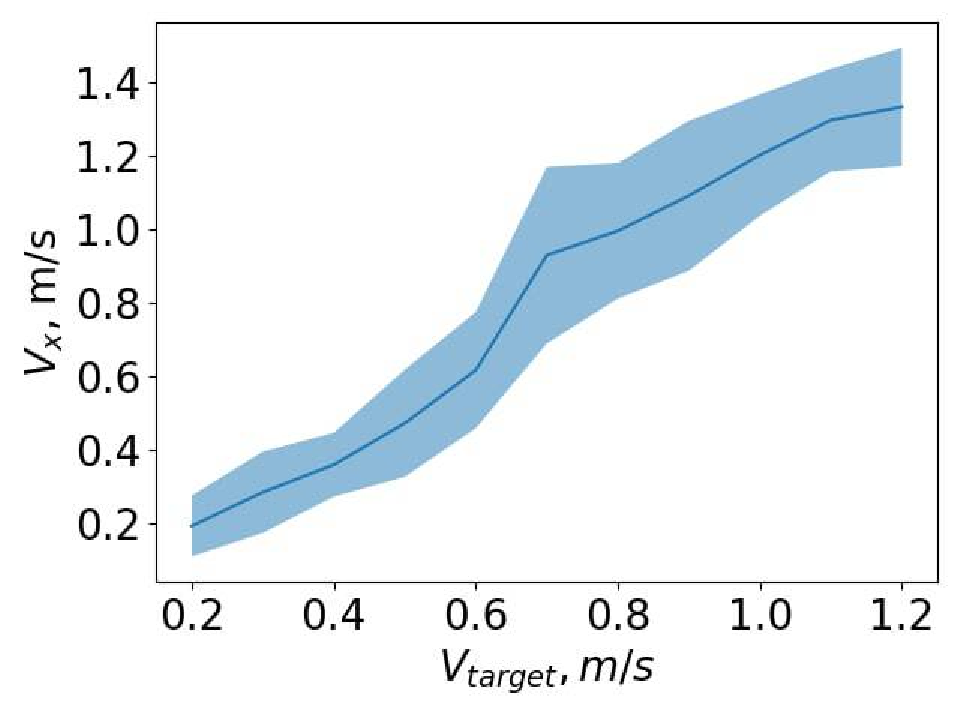
\includegraphics[width=1\textwidth]{images/vx}
\end{subfigure}%
\begin{subfigure}{.5\textwidth}
  \centering
  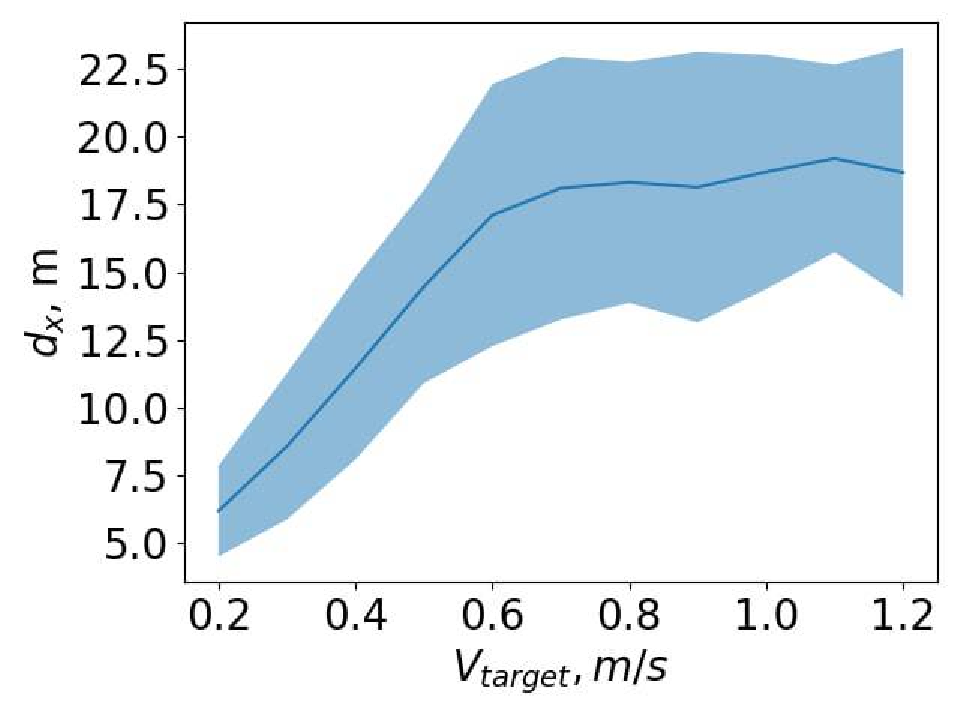
\includegraphics[width=1\textwidth]{images/dx}
\end{subfigure}%
\end{figure}
\begin{table} [htbp]
    \centering
    \begin{threeparttable}
        \begin{tabular}{| p{1cm} || p{2cm} | p{2cm} | p{2cm} |p{2cm} |}
            \hline
            \hline
            Задача & Вперед & Назад & По часовой & Против часовой \\
            \hline
            $R_{total}$ &	529 $\pm$ 124 &	508 $\pm$ 98 &	85 $\pm$ 219 &	165 $\pm$ 155 \\
            $N_{steps}$ & 3263 $\pm$ 633 &	3136 $\pm$ 545 &	2057 $\pm$ 1208 &	2095 $\pm$ 1325 \\
            \hline
            \hline
        \end{tabular}
    \end{threeparttable}
\end{table}
\end{frame}

\begin{frame}{Выводы}
\begin{itemize}
    \item Был разработан метод обучения робота Unitree A1 решать различные задачи перемещения
    \item Разработанная функция награды побуждает агента следовать плавной и безопасной стратегии
\end{itemize}
\end{frame}

%\begin{frame}
%    \frametitle{Четыре изображения}
%    \centering
%    \includegraphics[width=0.35\linewidth,angle=35]{latex}
%    \includegraphics[width=0.35\linewidth,angle=135]{latex}\\
%    \includegraphics[width=0.35\linewidth,angle=15]{latex}
%    \includegraphics[width=0.35\linewidth,angle=-15]{latex}
%\end{frame}

